\documentclass[a4paper]{article}

\usepackage[utf8]{inputenc}
\usepackage[spanish]{babel}
\usepackage[pdftex]{color,graphicx}
\usepackage{caption}
\usepackage{amsmath}
\usepackage{gensymb}
\usepackage{subcaption}
\usepackage{steinmetz}

\usepackage[pdftex,
	colorlinks=true,
	pdfauthor={Alejandro Vicario, Juan José Alberca},
	pdftitle={}]{hyperref}

\graphicspath{ {curvas/} }

\begin{document}

\title{Entregable 3 \\
\large TeleLabo 2018. Diseño de controladores}
\author{
	Juan José Alberca\\
	\texttt{jj.alberca@alumnos.upm.es}
	\and
	Alejandro Vicario\\
	\texttt{a.vicarioe@alumnos.upm.es}
}
\date{\today}


\maketitle


\section{Diferencia entre controladores}
\subsection{Seguimiento de señales de referencia monómicas}
En la función de transferencia de los controladores de segundo orden (P, P-D y PD), se puede comprobar que el numerador contiene un subpolinomio completo del denominador con grado $n_s=0$. Esto quiere decir que solo se resuelve el problema de seguimiento para señales monómicas de grado $q<1$, es decir, la señal escalón. Esto quiere decir que:
\begin{equation}
	e(\infty)=\lim_{s \rightarrow 0}
	s H(s) U(s) = 0
\end{equation}

Siendo $e(s)$ el error en la salida cuando en la entrada tenemos la función escalón $U(s)$. Con funciones de grado superior no se cumple esto: para la señal rampa se obtiene un error finito y para señales de mayor grado, error infinito.

Los controladores de tercer grado con un grado de libertad, que son PI, PID, PI-D, tienen un subpolinomio completo del denominador de grado $n_s=1$, por lo que además de poder resolver el problema de seguimiento con la señal escalón, también lo podrán resolver con la señal rampa. Es decir, lo podrán resolver para señales monómicas de grado $q<2$.
\begin{equation}
e(\infty)=\lim_{s \rightarrow 0}
s H(s) R(s) = 0, \textrm{con grado de } R(s)<2.
\end{equation}

Para los sistemas de dos grados de libertad estudiados existen dos posibilidades. En el sistema PID-D, al ser una generalización de los sistemas de tercer orden ya estudiados posee las mismas propiedades en el sentido del seguimiento de señales de referencia monómicas, es decir, hay error nulo para la rampa y error finito para la parábola. Pero si este sistema cumple la siguiente condición:
\begin{equation}
	K_P \tau_{D2} = -\frac{p}{K}
\end{equation}
también resuelve el problema de seguimiento para señales parabólicas.

 Por otro lado, el sistema D\textbar PID si es capaz de resolver parábola ya que el numerador contiene un subpolinomio completo del denominador con grado $n_s=3$.

\subsection{Comportamiento en régimen transitorio}
Para estudiar de forma más sencilla los controladores, en lugar de utilizar el parámetro de la constante proporcional, $K_p$, la constante de tiempo integral, $\tau_I$ y la constante de tiempo derivativa, $\tau_D$, se utilizan otros parámetros derivados de estos que resultan más intuitivos.
\begin{itemize}
	\item $\omega_n$: pulsación natural.
	\item $\zeta$: coeficiente de amortiguamiento. Se relaciona la velocidad con la que el sistema responde a una perturbación y con la amplitud de las oscilaciones que se pueden producir.
	\item $\beta$ y $\beta_2$: se relaciona con el tiempo que el sistema tarda en estabilizarse.
	\item $M_p$: sobreelongación máxima.
	\item $t_r$: tiempo de subida.
	\item $t_p$: tiempo de pico.
	\item $t_s$: tiempo de estabilización.
\end{itemize}
\subsubsection{Controladores P y P-D}
En un controlador P-D tenemos el parámetro de la rama proporcional $K_p$ y la constante de tiempo derivativa $\tau_D$. Su relación con $\beta_2$ y con $\zeta$ son las siguientes:
\begin{subequations}
	\begin{equation}
		\zeta= \frac{p+K_p K \tau_D}{\sqrt{2 K_p K}}
	\end{equation}
	\begin{equation}
		\tau_D= \frac{\zeta (2-\beta_2)}{\sqrt{K_p K}}
	\end{equation}
	\label{eq:1}
\end{subequations}
Como se puede observar, cuando $\beta_2=0$, se anula la rama derivativa, por lo que se comprueba que el controlador P es un caso particular del controlador P-D. Por lo tanto, comparten las características de régimen transitorio. Estas características corresponden con las de un sistema de segundo orden en su primera forma canónica. Debido a esto, en el controlador P-D es posible controlar $M_p$ de forma independiente a $t_p$, $t_r$ y $t_s$ mediante la variación de $K_p$ y $\tau_D$ según la ecuación \ref{eq:1}.

\subsubsection{Controladores PI, PID y PI-D}
Los controladores P, PD, P-D y PI son casos particulares de los controladores PID y PI-D. La razón de que el P y el PD se estudien por separado se debe a que su estudio matemático es posible y no es obligatorio realizar simulaciones, como ocurre con los otros.
Con estos controladores aparece el parámetro $\beta$ que procede de una escritura alternativa del polinomio característico de las funciones de transferencia de los mismos.

Las ganancias de los factores Derivativo e Integral de estos controladores vienen dadas por:
\begin{subequations}
	\begin{equation}
	K_D=K_P \tau_D
	\end{equation}
	\begin{equation}
	K_I=\frac{K_P}{\tau_I}
	\end{equation}
\end{subequations}

Ya que estos controladores no se pueden analizar de forma matemática es importante entender como afectan los parámetros del sistema $K_P$, $\tau_I$ y $\tau_D$ a sus polos. Estos nos darán la información sobre su comportamiento. Cuanto más lejos del origen se encuentre el polo, más rápido será el sistema respecto a cualquier cambio y cuanto más alejados entre sí estén los polos conjugados el controlador será más inestable y mayor será $M_p$. Este comportamiento está relacionado con la magnitud del coeficiente de amortiguamiento $\zeta$.

\subsubsection{Controladores PID-D y D\textbar PID}
Como los controladores PID-D son una generalización de los controladores PID y PI-D, para los que con $\tau_{D1}=0$ se obtiene un sistema PI-D y con $\tau_{D2}=0$ se obtiene un sistema PID.

Para analizar estos controladores se introducen los parámetros $r1$, $r2$, $r3$ que son funciones que dependen de $\beta$, $\zeta$ y $\omega_n$ de tal forma que si $frac{r1}{\omega_n}$, $\frac{r2}{\omega_n^2}$, $frac{r3}{\omega_n}$ son independientes de $\beta_2$, como en el caso del controlador PID-D y D\textbar PID, tendremos $M_p$ independiente de $\beta$, por lo que para diseñar estos controladores se puede seguir el mismo procedimientos que para diseñar los controladores PID y los PI-D.

\section{Análisis, diseño e implementación de un sistema de control de la posición angular de un motor DC, imponiendo especificaciones de régimen permanente y transitorio, utilizando un controlador D\textbar PID}
Se va a utilizar la siguiente función de transferencia:
\begin{equation}
G(s)=\frac{2652.28}{s(s+64.986)}
\end{equation}
\subsection{Análisis de estabilidad \label{estabilidad}}
Para estudiar la estabilidad del sistema primero debemos obtener el polinomio característico. Para un D\textbar PID es:
\begin{equation}
P(s)=s^3+(p+K K_P\tau_{D1})s^2+K K_P(s+\frac{1}{\tau_I})
\end{equation}
Donde:
\begin{itemize}
	\item $p$ es el polo del motor
	\item $K=K'/R$ con $R=23$ de la reductora
	\item $K_P$ es la constante de la rama proporcional
	\item $\tau_{D1}$ es la constante de tiempo derivativa de la rama principal
	\item $\tau_I$ es la constante de tiempo integral
\end{itemize}

Con el polinomio característico construimos la tabla de Routh:
\begin{center}
	\begin{tabular}{ccl}
		$s^3$: & $1$ & $K K_P$ \\ \\
		$s^2$: & $p+K K_P \tau_{D1}$ & $\displaystyle\frac{K K_P}{\tau_I}$ \\ \\
		$s^1$: & $\displaystyle\frac{K K_P (p+K K_P \tau_{D1} -\frac{1}{\tau_I})}{p+K K_P \tau_{D1}}$ & \\ \\
		$s^0$: & $\displaystyle\frac{K K_P}{\tau_I}$ &
	\end{tabular}
\end{center}

La condición necesaria para que el sistema sea estable es que no debe haber cambios de signo en la primera columna de la Tabla de Routh. Analizando los términos de la tabla se llegan a las siguientes condiciones.

Como 1 es positivo, el resto de parámetros deben ser positivos.
\begin{equation}
	p+K K_P \tau_{D1}>0
\end{equation}
Reorganizando,
\begin{equation}
	-\frac{p}{K}<K_P \tau_{D1}
	\label{eq:2}
\end{equation}
También debe cumplirse:
\begin{equation}
	\frac{K K_P (p+K K_P \tau_{D1} -\frac{1}{\tau_I})}{p+K K_P \tau_{D1}} > 0
\end{equation}
O lo que es lo mismo,
\begin{equation}
	\frac{1}{\tau_I} < p+K K_P \tau_{D1}
	\label{eq:3}
\end{equation}
Además se debe cumplir $\tau_I > 0$.

\subsection{Problema de seguimiento de las señales escalón, rampa y parábola}
La función de transferencia del controlador D\textbar PID tiene en su numerador un subpolinomio completo del denominador de grado 1. Por lo tanto, resuelve el problema de seguimiento para las funciones de grado $q<2$, es decir, para el escalón y la rampa.

Para comprobar que el controlador resuelve el problema de seguimiento para una señal determinada $R(s)$, se aplica el teorema del valor final sobre la señal de error del sistema.
La función de transferencia del error es,
\begin{equation}
	H_{e, D|PID}(s)=\frac{s^2(s+p-K K_P \tau_{D2})}{s^2(s+p)+K K_P \tau_{D1}(s^2+\frac{s}{\tau_{D1}}+\frac{1}{\tau_{D1} \tau_I})}
\end{equation}

Y tras aplicarle el teorema del valor final se obtiene:
\begin{equation}
	e(\infty)=\lim_{s \rightarrow 0}
	s H_{e, D|PID}(s) R(s)
\end{equation}

El límite tiende a 0 cuando $R(s)=\frac{1}{s}$ y para $R(s)=\frac{1}{s^2}$. Para que este error sea $0$ cuando $R(s)=\frac{1}{s^3}$, se debe cumplir la siguiente condición:
\begin{equation}
K_P \tau_{D2} = \frac{p}{K}
\end{equation}

\subsection{Cálculo de los parámetros del controlador según las condiciones dadas}
Puesto que la sobreelongación máxima $M_p$ es independiente de $\beta_2$, en primer lugar se va seleccionar un valor de $\beta_2$ y de $\zeta$ que cumpla con las especificaciones pedidas.
Para realizar este apartado se ha creado un código en Matlab que, dados unos valores de $\zeta$ y $\beta$, calcula la sobreelongación máxima a partir de la función de transferencia del sistema (Figura \ref{fig:mp}) que se da en la documentación de la asignatura:

\begin{equation}
	H_{D|PID}(s)=\frac{r_1 s r_2+}{s^2 + 2\zeta \omega_n s} + \frac{r_3}{s+ \beta \zeta \omega_n}
\end{equation}

\begin{subequations}
	\begin{equation}
		r_1 = \frac{\zeta(\beta(\frac{1}{\beta^2}-4)+\frac{2}{\zeta^2})}{Q(\beta)}
	\end{equation}
	\begin{equation}
		r_2 = \frac{\omega_n^2(\frac{1}{\zeta^2}-2\beta)}{Q(\beta)}
	\end{equation}
	\begin{equation}
		r_3=\frac{\beta^3 \zeta \omega_n}{Q(\beta)}
	\end{equation}
\end{subequations}
Donde $Q(\beta)=\beta^2-2 \beta + \frac{1}{\zeta^2}$.


\begin{figure*}[htp]
	\begin{center}
		\begin{subfigure}{1\textwidth}
			\centering
			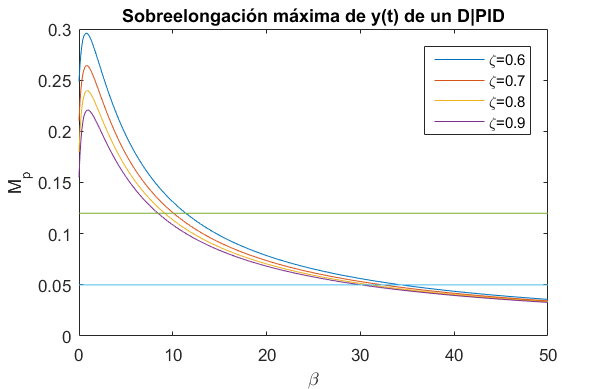
\includegraphics[width=12cm]{Mp3}
			\caption{Relación entre $Mp$ y $\beta$}
			\label{fig:mp}
		\end{subfigure}

		\begin{subfigure}{1\textwidth}
			\centering
			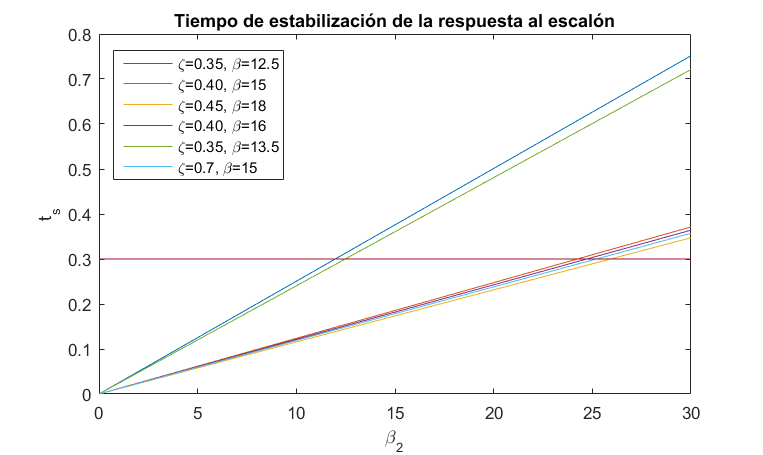
\includegraphics[width=12cm]{ts4}
			\caption{Relación entre $t_s$ y $\beta_2$}
			\label{fig:ts}
		\end{subfigure}
		\caption{}
	\end{center}
\end{figure*}

Una vez se han obtenido unos valores de $\zeta$ y $\beta$ que cumplan las especificaciones, se ha creado un código para calcular el tiempo de estabilización $t_s$ según el valor de $beta_2$ y la tolerancia $\nu$, y el resultado se muestra en la Figura \ref{fig:ts}.

Con este código y viendo las gráficas anteriores, se han elegido los valores que se han considerado más adecuados para las especificaciones pedidas. Se ha elegido una $M_P \approx 0.1$, lo que establece los valores de $\beta$ y de $\zeta$. A partir de estos valores, se realiza la simulación del tiempo de estabilización, que se ha elegido como $t_s = 0.05 s$, lo que establece el valor de $\beta_2$.

\begin{center}
	\begin{tabular}{c|c}
			$\beta$ & 15 \\
			$\beta_2$ & 3.5 \\
			$\zeta$ & 0.7 \\
	\end{tabular}
\end{center}

A partir de estos datos se pueden obtener $K_P$, $\tau_{D1}$, $\tau_{D2}$ y $\tau_I$ como se pide en el ejercicio, utilizando para ello las relaciones que se proporcionan en el documento de la asignatura.

\begin{subequations}
	\begin{equation}
		K_P=\frac{p^2(2\beta+\frac{1}{\zeta^2})}{\beta_2^2 K}
	\end{equation}
	\begin{equation}
		\tau_I=\frac{\beta_2^2*\zeta^2(2\beta + \frac{1}{\zeta^2})}{\beta p}
	\end{equation}
	\begin{equation}
		\tau_{D1}=\frac{\beta_2(\beta-\beta_2+2)}{p(2\beta + \frac{1}{\zeta^2})}
	\end{equation}
	\begin{equation}
		\tau_{D2}=\frac{p}{K K_P}
	\end{equation}
\end{subequations}

Cuyos resultados son:
\begin{center}
	\begin{tabular}{c|c}
		$K_P$ & 95.9556 \\
		$\tau_I$ & 0.0564 \\
		$\tau_{D1}$ & 0.0227 \\
		$\tau_{D2}$ & 0.0059 \\
	\end{tabular}
\end{center}

Para asegurar la validez de estos datos, se va a analizar la estabilidad del sistema a través de método de la tabla de Routh, descrito en el apartado \ref{estabilidad}.
Calculando, en la ecuación \ref{eq:2}:
\begin{equation}
	-\frac{64.986}{2652.28}< 95.9556\cdot0.0227 \Rightarrow
	-0.0245<2.178
\end{equation}
En la ecuación \ref{eq:3}:
\begin{equation}
	\frac{1}{0.0564} < 64.986+2652.28\cdot95.9556\cdot0.0227 \Rightarrow
	17.73<5842.161
\end{equation}
Además, se cumple que $\tau_I > 0 \Rightarrow 0.0564>0$.

Como se aprecia, todas las condiciones se cumplen, por lo que el sistema es obviamente estable y los valores obtenidos son válidos.

\subsection{Prueba del sistema diseñado en Telelabo \label{sec:pruebas}}
Para realizar las pruebas del sistema, primero se han tenido que calcular los valores de los parámetros para introducirlos en el programa. Estos también se han calculado en Matlab, utilizando las siguientes relaciones:
\begin{equation}
K_I=\frac{K_p}{\tau_I} T_s
\end{equation}
\begin{equation}
K_{Di}=\frac{K_P \tau_{Di}}{T_s}, i=1,2
\end{equation}
En las pruebas se ha usado un valor de periodo de muestreo $T_s=5$.

Los valores obtenidos son:
\begin{center}
	\begin{tabular}{c|c}
		$K_P$ & 95.9556 \\
		$K_I$ & 8.5111 \\
		$K_{D1}$ & 435.4904 \\
		$K_{D2}$ & 112.9049 \\
	\end{tabular}
\end{center}

Se han realizado pruebas para diferentes entradas: escalón, rampa y parábola, como se aprecian en la figura \ref{respuestas}.
En las tres gráficas se puede comprobar como el error en régimen permanente tiende a $0$.

\begin{figure*}[htp]
	\begin{subfigure}{1\textwidth}
		\centering
		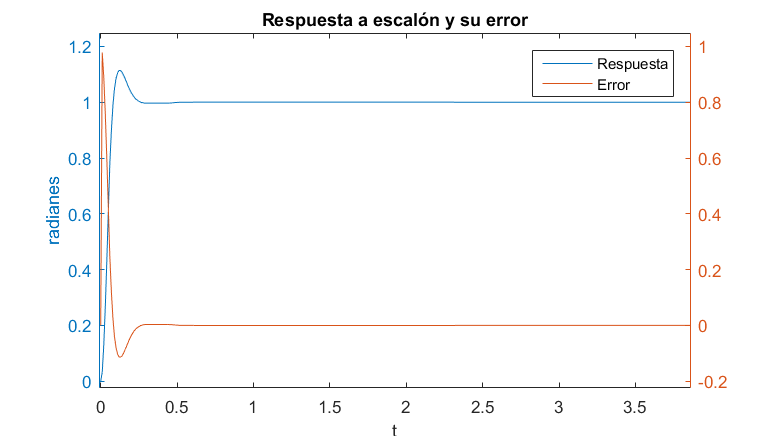
\includegraphics[width=10cm]{step2}
		\caption{Respuesta al escalón}
		\label{fig:step}
	\end{subfigure}

	\begin{subfigure}{1\textwidth}
		\centering
		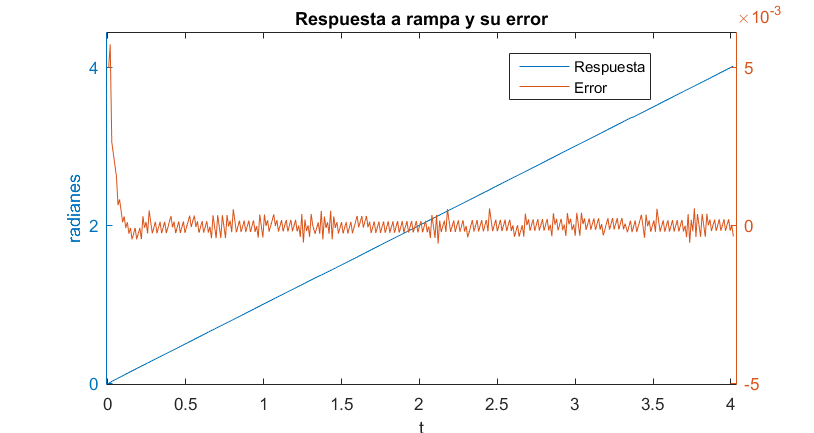
\includegraphics[width=10cm]{ramp2}
		\caption{Respuesta a la rampa}
		\label{fig:ramp}
	\end{subfigure}

	\begin{subfigure}{1\textwidth}
		\centering
		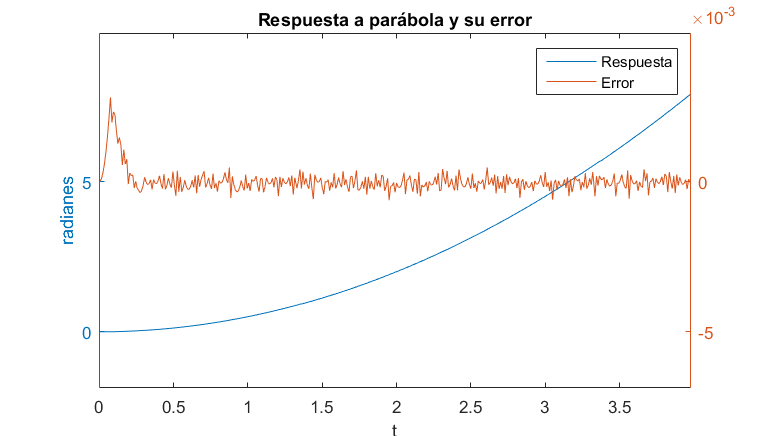
\includegraphics[width=10cm]{parab2}
		\caption{Respuesta a la parábola}
		\label{fig:parab}
	\end{subfigure}
	\caption{}
	\label{respuestas}
\end{figure*}


Teniendo en cuenta la respuesta al escalón, se han calculado los valores de $M_P$, $t_r$ y $t_s$ tras observar las gráficas de Matlab de la Figura \ref{fig:step} en detalle.

\begin{figure*}[htp]
	\begin{center}
		\begin{subfigure}[b]{0.45\textwidth}
			\centering
			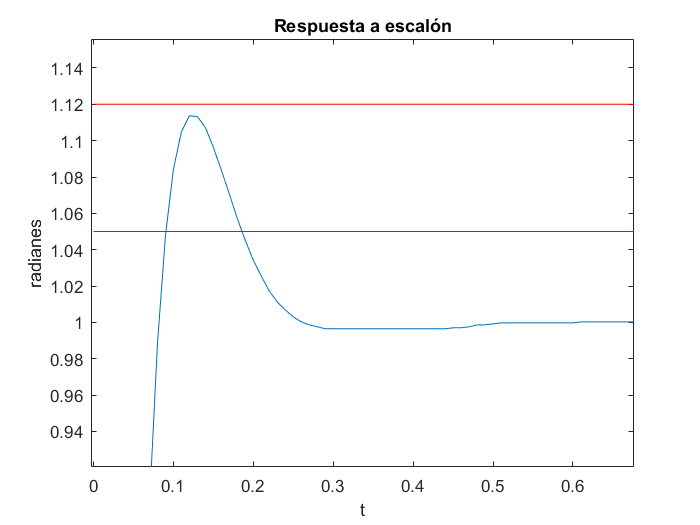
\includegraphics[width=\textwidth]{escalon_Mp2}
			\caption{Detalle valor de $M_P$}
			\label{mp2}
		\end{subfigure}
		\begin{subfigure}[b]{0.45\textwidth}
			\centering
			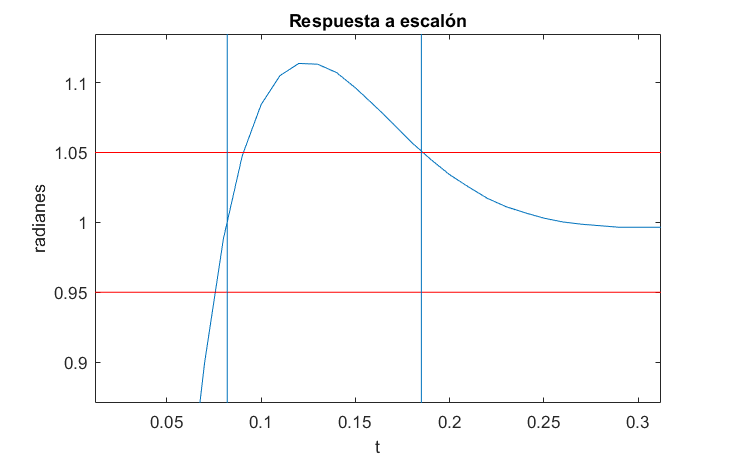
\includegraphics[width=\textwidth]{escalon_ts_tr2}
			\caption{Detalle valores de $t_s$ y $t_r$}
			\label{fig:tr}
		\end{subfigure}
	\end{center}
		\caption{Análisis de la respuesta al escalón del motor}
		\label{fig:escalon}
	\end{figure*}

De la figura \ref{mp2} se obtiene el valor de la sobreelongación máxima, que es aproximadamente $M_P=1.114$. El tiempo de subida y el tiempo de estabilización, $t_r=0.081 s$ y $t_s=0.185 s$, que se obtienen de la figura \ref{fig:tr}.

Los valores obtenidos cumplen con las especificaciones que se piden en el ejercicio, aunque difieren ligeramente de los valores calculados teóricamente y mediante simulaciones. Esto probablemente se deba a las no linealidades del motor, rozamiento, saturación del controlador y la dependencia con el periodo de muestreo.

\section{Análisis, diseño de un controlador PID en el lazo directo sintonizado en el dominio de la frecuencia mediante el método de Ziegler-Nichols Modificado}
Se utiliza la función de transferencia:
\begin{equation}
G(s)=\frac{22233201,58/23}{s(s+8382,70)(s+64.986)}
\end{equation}
\subsection{Análisis del motor en el Dominio de la Frecuencia}
Para realizar este análisis se ha obtenido el diagrama de Bode y el diagrama de Nyquist en Matlab que se pueden ver en la Figura \ref{bode}. En el diagrama de Bode se han marcado de forma aproximada los dos polos.


\begin{figure}[htp]
	\begin{subfigure}{1\textwidth}
		\centering
		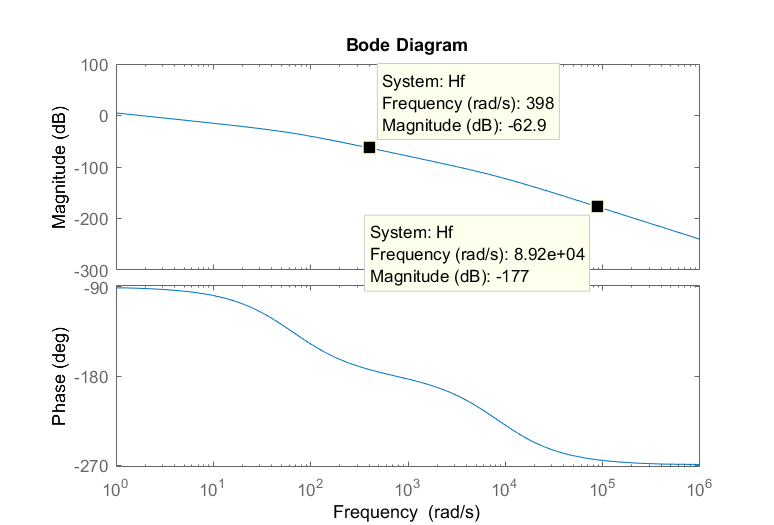
\includegraphics[width=\textwidth]{bode}
		\caption{Diagrama de Bode}
	\end{subfigure}

	\begin{subfigure}{1\textwidth}
		\centering
		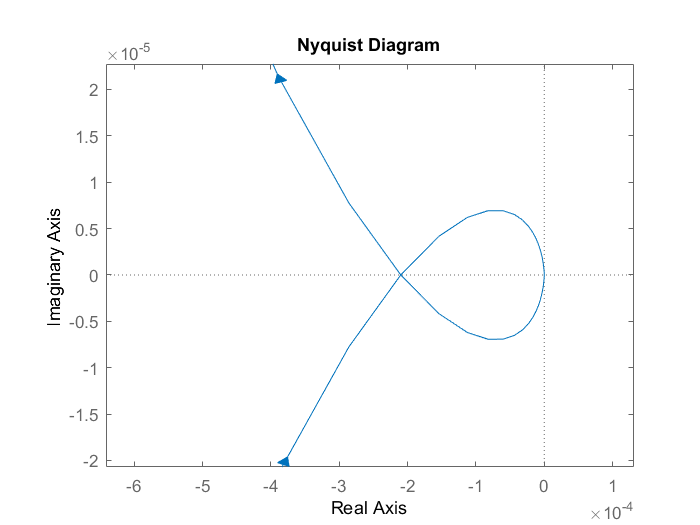
\includegraphics[width=\textwidth]{nyquist}
		\caption{Diagrama de Nyquist}
	\end{subfigure}
	\caption{Representación de la función de transferencia del motor}
	\label{bode}
\end{figure}


En el diagrama de Nyquist se puede apreciar como en el origen hay un valor de ganancia infinita y una fase de -90\degree  debido al primer polo de la función de transferencia. Esto es así debido a que cuando se analiza la posición angular del motor, este se comporta como un sistema integrador. Después, a medida que aumenta la frecuencia, la ganancia disminuye hasta que se llega al polo, donde la fase se ha retrasado 45\degree  más. Cuando se produce el cruce con el eje, hay -180\degree  en la fase, que se corresponden con una década más. Después de este primer polo, el módulo de la función de transferencia disminuye más rápido, por lo que aumenta aún más la curvatura del diagrama hacia el origen. Al haber otro polo más, el diagrama pasa por debajo del eje real ya que este está situado en -235\degree. Este polo provoca que la función de transferencia en el infinito tenga una fase de -270\degree.

Como se puede apreciar estamos ante un sistema integrador que sería inestable frente a una referencia en lazo abierto. En ese caso, si se introduce una señal de referencia constante la salida crecería hacia el infinito de forma descontrolada. Por eso es necesario un sistema de lazo cerrado.

\subsection{Diseño de un controlador PID mediante el método de  Ziegler-Nichols Modificado}
Desde el punto de vista de la frecuencia, un controlador PID desplaza los puntos del diagrama de Nyquist de tal forma que, ajustando los valores del controlador, se puede variar la forma del diagrama de Nyquist y por lo tanto los parámetros que forman el mismo para conseguir el sistema deseado.

Se puede estudiar el comportamiento del motor en lazo cerrado, descrito en la siguiente ecuación, cuyo resultado se muestra en la figura \ref{fig:cl}.

\begin{equation}
H_{CL}(s)=\frac{G(s)}{1 + G(s)}
\end{equation}


\begin{figure}[htp]
	\centering
	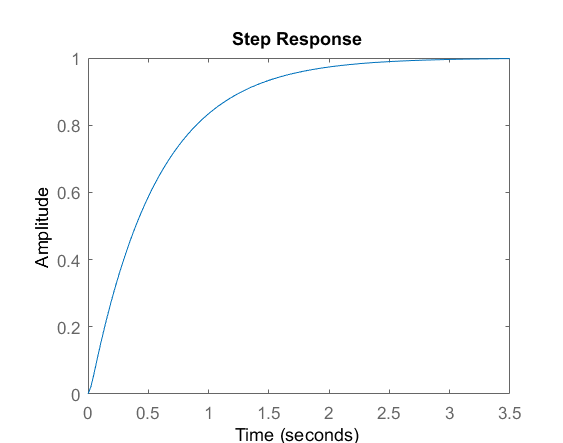
\includegraphics[width=7cm]{lazo_cerrado}
	\caption{Respuesta del motor en lazo cerrado a un escalón unitario.}
	\label{fig:cl}
\end{figure}


Como el diagrama de Nyquist del motor corta la circunferencia unidad con un ángulo cercano a 90\degree, se ha elegido utilizar un margen de fase menor, $M.F. = 30\degree$, para así reducir el tiempo de respuesta pero sin comprometer la estabilidad. Se han tenido en cuenta los resultados obtenidos en la sección \ref{sec:pruebas} para escoger la sobreelongación máxima y el tiempo de estabilización. $M_P=50\%$ y $t_s=10 s$, con una tolerancia del $5\%$. Estos márgenes son tan holgados debido a que se pretende centrarse en la respuesta en frecuencia del controlador en lugar de en su respuesta temporal. Además, se va a tener en cuenta también que el error frente a una perturbación constante debe ser nulo.

Para cumplir estas especificaciones se va a elegir el punto de corte del diagrama de Nyquist del motor en lazo abierto con la circunferencia unidad, $A=G(j\omega_0)$,
con $\omega_0 = 1.77 rad/s$ y se va a desplazar al punto $B=G_C(j\omega_0) G(j\omega_0)$, que también corta la circunferencia unidad pero en el punto donde $M.F. = 30\degree$.


\begin{subequations}
	\begin{equation}
		A=G(j\omega_0)=1 \phase{88.42\degree}
	\end{equation}
	\begin{equation}
		B=G_C(j\omega_0) G(j\omega_0)= 1 \phase{30\degree}
	\end{equation}
\end{subequations}

Para realizar estas transformaciones sería suficiente usar un controlador PI, pero debido al controlador pedido se usan las ecuaciones para un sistema PID descritas por el método de Ziegler-Nichols modificado.

\begin{subequations}
	\begin{equation}
		K_p=r_c cos \phi_c
	\end{equation}
	\begin{equation}
		\tau_D = \alpha \tau_I
	\end{equation}
	\begin{equation}
		\tau_I=\frac{tg\phi_c + \sqrt{4\alpha+tg^2\phi_c}}{2\omega_0\alpha}
	\end{equation}
\end{subequations}


Si se elige una $\alpha = 0.25$ se obtienen los siguientes parámetros:

\begin{subequations}
	\begin{equation}
		K_p = 0.5236
	\end{equation}
	\begin{equation}
		\tau_D = 0.0797
	\end{equation}
	\begin{equation}
		\tau_I= 0.3188
	\end{equation}
\end{subequations}

Con estos parámetros se puede describir el sistema en lazo cerrado:

\begin{equation}
G_C(s)=K_P (1 + s \tau_D + \frac{1}{s\tau_I})
\end{equation}

\begin{equation}
H(s)=\frac{G_C(s) G(s)}{1 + G_C(s) G(s)}
\end{equation}

Cuyo diagrama de Nyquist y respuesta al escalón se puede ver en la figura \ref{fig:sim} y se pueden comprobar que $M_P=47\%$ y $t_s=6.17 s$, cumpliendo las especificaciones de diseño. Además se obtiene el $M.F. = 30\degree$ deseado y un margen de ganancia infinito.


\begin{figure}[htp]
	\begin{center}
		\begin{subfigure}[b]{0.45\textwidth}
			\centering
			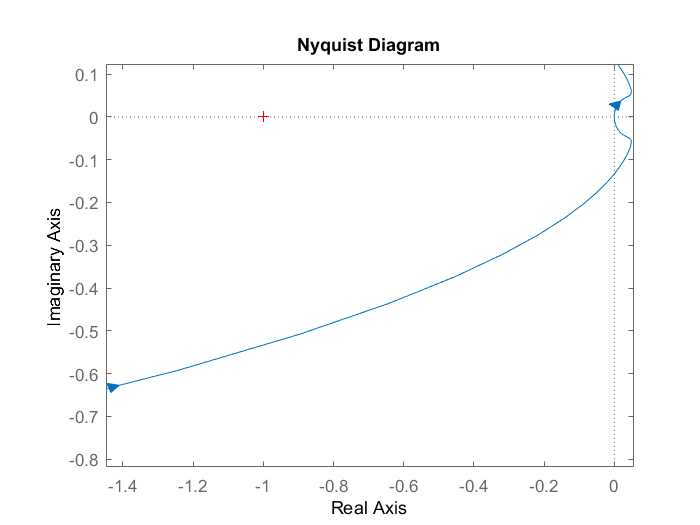
\includegraphics[width=\textwidth]{nyquist2}
			\caption{Diagrama de Nyquist}
		\end{subfigure}
		\begin{subfigure}[b]{0.45\textwidth}
			\centering
			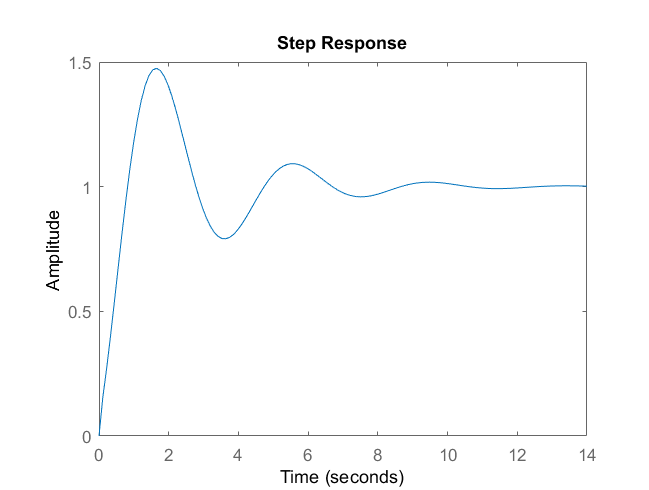
\includegraphics[width=\textwidth]{respuesta}
			\caption{Respuesta al escalón}
			\label{escalonteorico}
		\end{subfigure}
	\end{center}
	\caption{}
	\label{fig:sim}
\end{figure}


\subsection{Prueba del sistema diseñado en Telelabo}

Para calcular los parámetros que se introducen en el software del Telelabo, se han utilizado las siguientes relaciones:
\begin{equation}
	K_I=\frac{K_p}{\tau_I} T_s
\end{equation}

\begin{equation}
	K_{D}=\frac{K_P \tau_{D}}{T_s}
\end{equation}

En las pruebas se ha usado un valor de periodo de muestreo $T_s=5$.


Los valores obtenidos son:
\begin{center}
	\begin{tabular}{c|c}
		$K_P$ & 0.524 \\
		$K_I$ & 0.008 \\
		$K_{D}$ & 8.346 \\
	\end{tabular}
\end{center}

Teniendo en cuenta la respuesta al escalón de la figura \ref{real}, se han obtenido los valores reales de $M_P = 40\% $ y $t_s = 9.5 s$.
Además, como el diseño está enfocado a la respuesta en frecuencia, se ha realizado el experimento de respuesta un seno a la pulsación característica $\omega_0 = 1.77 rad/s$ del sistema realizado, cuya salida puede verse en la figura \ref{seno}.
En este experimento se ha medido la amplitud y el desfase del seno resultante. Los valores teóricos de estos parámetros en el caso de un sistema realimentado, con un margen de fase $M.F = 30\degree$ y una ganancia unidad en la pulsación caracteristica son:

\begin{subequations}
	\begin{equation}
		Amp = 2 G_C(j\omega_0) G(j\omega_0) = 2
	\end{equation}
	\begin{equation}
		\phi = \frac{-180\degree+M.F}{2} = -75\degree
	\end{equation}
\end{subequations}

Tras realizar el experimento en el Telelabo los valores obtenidos son: $Amp = 1.5$ y $\phi \approx 85\degree$, los cuales difieren apreciablemente del sistema teórico.
Sin conocer exactamente la implementación del controlador en el laboratorio, según la figura \ref{real}, parece que hubiera algún tipo de saturación en el sistema, probablemente de la parte integral, que provoca una distorsión que modifica el resultado del experimento.

\begin{figure*}[htp]
	\centering
	\begin{subfigure}{0.45\textwidth}
		\centering
		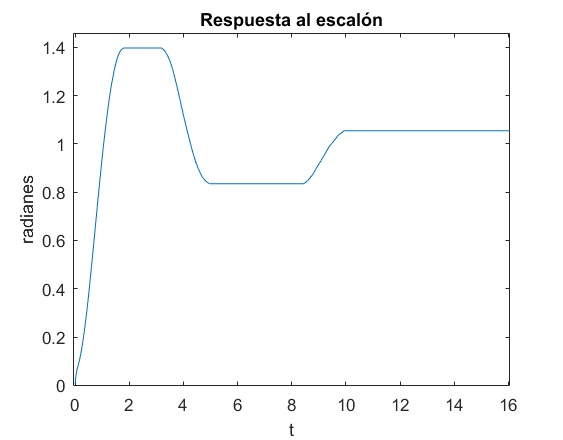
\includegraphics[width=\textwidth]{respuesta_labo}
		\caption{Respuesta al escalón}
		\label{escalonreal}
	\end{subfigure}
	\begin{subfigure}{0.45\textwidth}
		\centering
		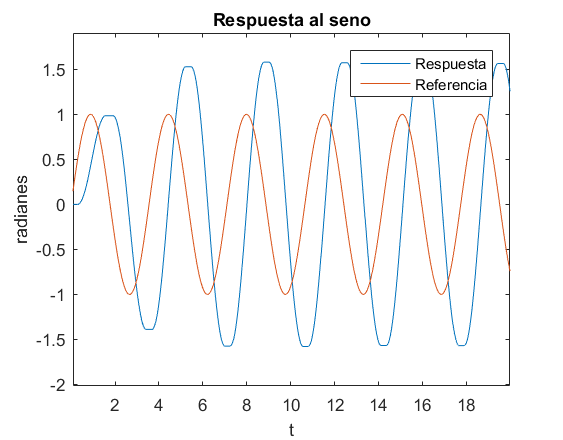
\includegraphics[width=\textwidth]{respuesta_seno}
		\caption{Respuesta al seno}
		\label{seno}
	\end{subfigure}
	\caption{Resultados a experimentos reales en el Telelabo}
	\label{real}
\end{figure*}

\section{Conclusiones}

Con este trabajo se han seguido dos métodos de diseño diferentes basados en controladores: uno teniendo en cuenta el dominio de la frecuencia y otro bajo condiciones específicas de régimen permanente y transitorio.
En ambos casos, los resultados obtenidos de forma teórica y matemática no coinciden del todo con las pruebas reales realizadas en el motor, a pesar de que cumplen con las especificaciones pedidas en el enunciado.
Esto puede deberse a diversos factores, por una parte, el propio motor no es ideal, ya que existe un rozamiento, dependencias con la temperatura y con las condiciones ambientales, saturación, inexactitudes en su fabricación o desgaste del mismo., por ejemplo, pueden afectar al valor final de las pruebas.
Por otra parte, existen también efectos causados por el software que lo controla.

Estos últimos son los que ha resultado más interesantes. Por una parte, todo el desarrollo matemático se realiza para un sistema en tiempo continuo, sin embargo el sistema del TeleLabo, como cualquier equipo informático, opera en tiempo discreto, lo que obligaba a introducir el parámetro del tiempo de muestreo.
Aunque en el desarrollo teórico este parámetro solo se tenía en cuenta al final, era facil comprobar que el sistema controlador no era independiente de este, llegando a casos en los que, por ejemplo, el sistema se volvía estable o inestable dependiendo de este parámetro.

También ha sido interesante descubrir como el motor se "paraba" en algunos momentos, como en la figura \ref{escalonreal}, sin causa aparente, provocando algo parecido a una saturación. Este efecto no se puede estudiar en profundidad sin conocer la implementación del sistema controlador, pero muy probablemente sea debido a la saturación de algún valor interno del sistema, seguramente de la parte integral.

EN definitiva, lo que se ha podido aplicar en el desarrollo de la práctica, es que a pesar de las no idealidades que pueda tener un sistema cualquiera, si se trabaja dentro de unos rangos determinados y se guardan una serie de precauciones, es posible que los sistemas teóricos obtengan resultados muy similares a su implementación real, lo que es tremendamente útil, ya que es posible trabajar de forma mucho más eficiente con ellos.


\begin{thebibliography}{9}
\bibitem{git} \href{https://github.com/avicarioe/telelabo}{Repositorio del proyecto alojado en GitHub}
\bibitem{design} Félix Monasterio-Huelin y Álvaro Gutiérrez Martín;
\href{http://www.robolabo.etsit.upm.es/asignaturas/seco/apuntes/design.pdf}{Diseño}
\bibitem{routh} John Wiley \& Sons, Inc; Norman S. Nise. Control Systems Engineering.
\bibitem{frecuencia} Félix Monasterio-Huelin y Álvaro Gutiérrez Martín;
\href{http://robolabo.etsit.upm.es/asignaturas/seco/apuntes/frecuencia.pdf} {Frecuencia}


\end{thebibliography}

\end{document}
